% main.tex
\documentclass[conference]{IEEEtran}

\usepackage[T1]{fontenc}
\usepackage{lmodern}
\usepackage{microtype}
\usepackage{graphicx}
\usepackage{amsmath,amssymb}
\usepackage{booktabs}
\usepackage{multirow}
\usepackage{array}
\usepackage{cite}
\usepackage{url}
\usepackage{xcolor}
\usepackage[hidelinks]{hyperref}
\usepackage{xspace}

\usepackage{tikz}
\usetikzlibrary{arrows.meta,positioning,fit,calc,shapes.geometric,shapes.misc,shapes.symbols}

\usepackage{algorithm}
\usepackage{algpseudocode}

\usepackage{balance} % balances references columns on last page

\interdisplaylinepenalty=2500

\newcommand{\cgp}{Commons Guild Protocol (CGP)\xspace}
\newcommand{\atproto}{AT Protocol\xspace}
\newcommand{\ssb}{Secure Scuttlebutt (SSB)\xspace}

% --- TikZ styles ---
\tikzset{
  box/.style={rounded corners, draw, thick, align=center, inner sep=6pt, font=\footnotesize},
  pill/.style={rounded corners=9pt, draw, thick, align=center, inner sep=5pt, font=\footnotesize},
  db/.style={cylinder, shape border rotate=90, aspect=0.25, draw, thick, align=center, inner sep=5pt, font=\footnotesize},
  arr/.style={-{Latex[length=2.4mm]}, thick},
  darr/.style={-{Latex[length=2.4mm]}, thick, dashed},
  small/.style={font=\footnotesize},
}

\title{\cgp: Tokenless, Forkable, Guild-Centric Communication with\\
Verifiable Logs and Role-Based Relays}

\author{%
\IEEEauthorblockN{Ryan Hardesty Lewis}%
\IEEEauthorblockA{Institute for Data, Systems, \& Society, MIT}%
}

\begin{document}
\maketitle

\begin{abstract}
Modern real-time communities largely rely on centralized platforms, where a single operator controls governance, moderation, and data retention. Decentralized alternatives exist, but they typically optimize for different primitives---identity-centric feeds, global firehoses, or federated DAG state---which introduces a mismatch when building communities at scale. This paper introduces \cgp, a draft protocol for tokenless, forkable, guild-centric chat built on append-only signed logs inspired by hash chains and transparency systems. \cgp deliberately avoids mandatory proof-of-work, mining, or per-message fees, and instead supports \emph{optional relay plugins} (e.g., anti-spam puzzles, proof-of-compression, media pinning, or on-chain anchoring). A key architectural choice is a \emph{role-based relay architecture} with separable discovery and data roles: (i) independent \emph{directory operators} act in a discovery role, maintaining transparency logs that map human-readable handles to guild identifiers and relay endpoints; and (ii) separate \emph{guild relays} sequence and serve each guild's event log, with additional relay roles as needed. We analyze trade-offs relative to Matrix, \ssb, \atproto/Bluesky, Nostr, and Push Protocol, and outline extensions for verifiable checkpointing, scalable media handling, and optional proofs.
\end{abstract}

\begin{IEEEkeywords}
decentralized communication, transparency logs, Merkle trees, append-only logs, governance, forkability, guild chat, content addressing
\end{IEEEkeywords}

\section{Introduction}
Centralized chat systems deliver excellent user experience but concentrate control over identity, moderation, and history. Discord popularized \emph{guilds} (servers), \emph{channels}, and \emph{roles} as the primary mental model, yet its data plane and governance ultimately depend on a single operator \cite{discordGuild}. 

Decentralized protocols span a wide design space. Matrix federates rooms across independently operated servers and resolves shared room state over an event DAG \cite{jacob2020matrixdecomposition}. \ssb replicates identity-centric append-only feeds peer-to-peer \cite{tarr2019ssb}. The \atproto separates personal data servers (PDS), relays, and app views for social applications \cite{kleppmann2024atproto}. Nostr publishes signed events to relays with optional conventions \cite{wei2024nostr}. Push Protocol roots messaging in Web3 primitives and chain-centric assumptions \cite{pushLitepaper}. Yet each of these systems is tuned to a different core primitive (global feeds, social graphs, or chain-centric messaging).


This paper introduces \cgp, a \emph{tokenless} and \emph{PoW-optional} group chat protocol that borrows Bitcoin-inspired tamper-evident data structures (hash chains and Merkle roots) \cite{nakamoto2008bitcoin,merkle1987}. \cgp keeps message payloads off-chain while allowing optional anchoring for auditability. The base standard is intentionally minimal: it mandates only core integrity invariants and wire compatibility, while relay operators can layer additional policies---such as ephemerality, anti-spam proofs, compression budgets, or media pinning---without fragmenting interoperability.

\section{Design Goals and Non-goals}
\subsection{Goals}
\textbf{G1: Guild-first model.} Guilds, channels, and roles are first-class, so clients get server/room semantics directly instead of encoding them into per-user feeds or DAGs.

\textbf{G2: Tamper-evident history without blockchain dependence.} A guild is an append-only signed event log with hash-linked structure. Clients can verify integrity locally without requiring a blockchain.

\textbf{G3: Forkable governance.} Communities can fork a guild's history at a known checkpoint and continue under new rules or operators (analogous to software forks, inspired by the social dynamics of ledger forks \cite{nakamoto2008bitcoin}).

\textbf{G4: Transparent, role-based discovery.} Usernames resolve through directory operators that maintain Merkle-based transparency logs (in the spirit of Certificate Transparency \cite{rfc6962}) and are cleanly separated from guild relays.

\textbf{G5: Thin clients and selective sync.} Browsers and mobile clients should sync only the guilds and channels they care about, with configurable retention windows.

\subsection{Non-goals}
\textbf{N1: Global consensus.} \cgp does not attempt to maintain a single canonical world state, unlike blockchains.

\textbf{N2: Exactly-once delivery.} The protocol targets eventual consistency with at least one honest relay.

\textbf{N3: Mandatory end-to-end encryption.} Payload encryption can be layered on top (e.g., using Signal-style primitives \cite{doubleRatchet}), but it is not required by the format.

\section{Architecture Overview}
\subsection{Role-based relay architecture}
\cgp organizes the network into orthogonal \emph{relay roles}, as seen in Figure \ref{fig:overview}. In the simplest deployment we highlight two:

\vspace{0.2cm}

(1) a \textbf{discovery role}, in which multiple directory operators maintain \emph{transparency logs} that map a handle (e.g., \texttt{@soulsborne/pvp}) to a guild identifier, public key, and relay descriptors

\vspace{0.2cm}

(2) a \textbf{guild role}, in which one or more guild relays store and serve the guild log and provide sequencing for events.

\vspace{0.2cm}

Additional relay roles (e.g., media storage, anti-abuse, or archival relays) can be added without changing the core log format. This role-based separation decouples \emph{finding} a guild from \emph{hosting} its history, and avoids forcing a single global feed-aggregator architecture (e.g., relay-driven ``firehose'' distribution in AT-Protocol-style systems \cite{kleppmann2024atproto}) for chat-style selective participation.


\begin{figure}[t]
\centering
\resizebox{\columnwidth}{!}{%
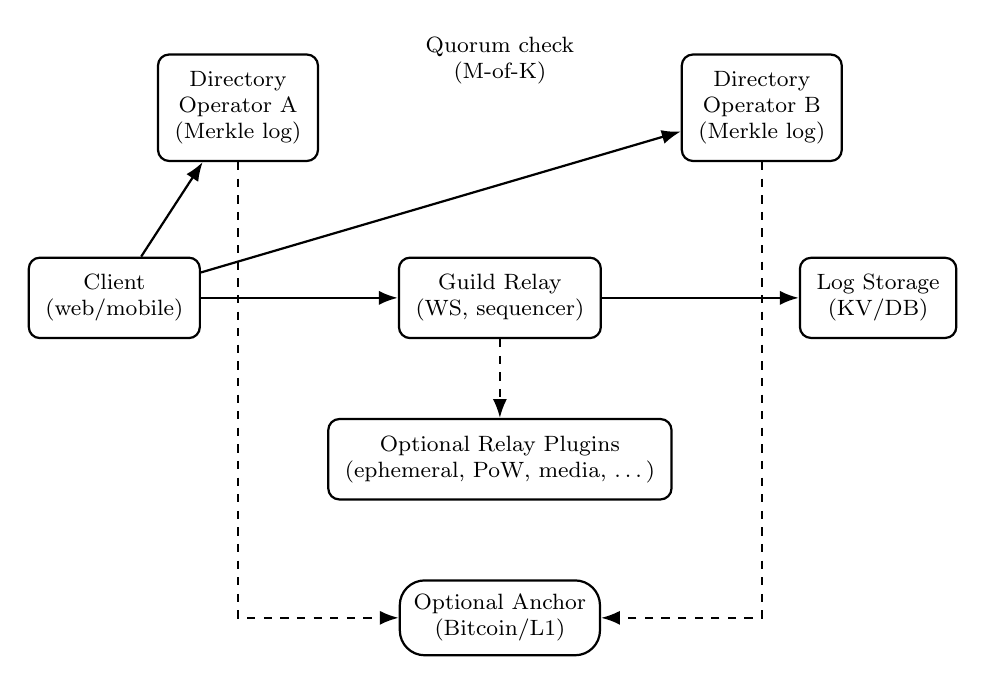
\begin{tikzpicture}[node distance=10mm]

\node[box] (client) {Client\\(web/mobile)};
\node[box, right=25mm of client] (guildrelay) {Guild Relay\\(WS, sequencer)};
\node[box, right=25mm of guildrelay] (storage) {Log Storage\\(KV/DB)};

\node[box, above left=12mm and 10mm of guildrelay] (dir1) {Directory\\Operator A\\(Merkle log)};
\node[box, above right=12mm and 10mm of guildrelay] (dir2) {Directory\\Operator B\\(Merkle log)};

\node[box, below=10mm of guildrelay] (plugins) {Optional Relay Plugins\\(ephemeral, PoW, media, \ldots)};
\node[pill, below=10mm of plugins] (anchor) {Optional Anchor\\(Bitcoin/L1)};

% arrows (no labels, no curves)
\draw[arr]  (client)      -- (guildrelay);
\draw[arr]  (client)      -- (dir1);
\draw[arr]  (client)      -- (dir2);

\draw[arr]  (guildrelay)  -- (storage);
\draw[darr] (guildrelay)  -- (plugins);

\draw[darr] (dir1) |- (anchor);
\draw[darr] (dir2) |- (anchor);

\node[small, align=center] at ($(dir1)!0.5!(dir2) + (0,6mm)$) {Quorum check\\(M-of-K)};

\end{tikzpicture}%
}
\caption{System overview. Directory operators provide transparency-backed discovery; guild relays sequence and serve logs; optional anchoring and relay plugins add policy without breaking core interoperability.}
\label{fig:overview}
\end{figure}



\subsection{Guild log as a verifiable append-only structure}
A guild is defined by its genesis event. Subsequent events increment a sequence number and include the previous event hash, forming a hash chain \cite{nakamoto2008bitcoin}. Each event is signed using secp256k1 parameters standardized by SEC~2 \cite{sec2}, with optional Schnorr signatures \cite{schnorr1991}.

\subsection{Directory transparency logs}
Directory operators provide \emph{inclusion proofs} and \emph{consistency proofs} (Figure \ref{fig:directory}), mirroring transparency-log approaches \cite{rfc6962}. Clients consult multiple operators and require a quorum agreement to reduce reliance on any single naming authority. Directory operators become auditable log witnesses rather than a single trusted registrar.

\begin{figure}[t]
\centering
\resizebox{\columnwidth}{!}{%
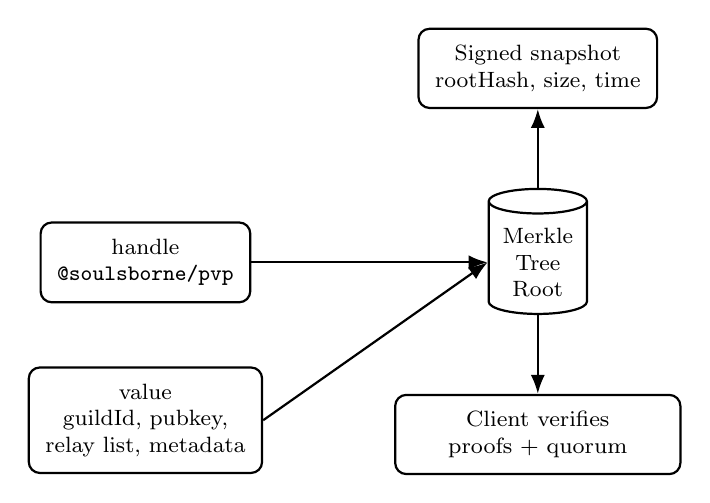
\begin{tikzpicture}[node distance=8mm]

\node[box] (h) {handle\\\texttt{@soulsborne/pvp}};
\node[box, below=8mm of h] (v) {value\\guildId, pubkey,\\relay list, metadata};

\node[db, right=30mm of h] (mtree) {Merkle\\Tree\\Root};
\node[box, above=10mm of mtree] (snap) {Signed snapshot\\rootHash, size, time};
\node[box, below=10mm of mtree, text width=3.2cm] (client)
  {Client verifies\\proofs + quorum};

% arrows (simple, straight / L-shaped, no labels)
\draw[arr] (h.east) -- (mtree.west);
\draw[arr] (v.east) -- (mtree.west);

\draw[arr] (mtree) -- (snap);
\draw[arr] (mtree) -- (client);

\end{tikzpicture}%
}
\caption{Directory operators commit mappings into Merkle trees and sign snapshots, enabling inclusion and consistency proofs.}
\label{fig:directory}
\end{figure}

\section{Core: Events, Verification, and Sync}
\subsection{Wire model}
The reference transport is WebSocket \cite{rfc6455}, using simple JSON array frames, similar in spirit to Nostr's relay framing \cite{wei2024nostr}. Relays advertise optional \texttt{features} during handshake, allowing clients to adapt without hard-forking the protocol.

\subsection{Event verification}
Clients and relays reject events that violate the following conditions: monotonic \texttt{seq}; correct \texttt{prevHash}; valid \texttt{id = SHA256(canonical(event))}; and a valid signature under the author key (secp256k1 \cite{sec2}).

\subsection{Computing channel state}
Channel state is derived deterministically by replaying the log. A \texttt{MESSAGE} event creates a message; \texttt{DELETE} removes it; and \texttt{EDIT} updates the visible representation. This yields a simple ``UTXO-like'' model (create/spend/update) without requiring full DAG state resolution.

\section{Governance and Forkability}
A core differentiator of \cgp is explicit, protocol-level support for \emph{forking}. A fork event references a parent guild, a parent sequence number, and the parent root hash, enabling clients to render lineage and verify the fork point.

Forkability reframes moderation disputes as \emph{exit rights}: communities can migrate to new relays or new rule sets while keeping cryptographic continuity with the original history. In practice, this lets users keep their history without being locked into any one operator’s governance.

\section{Comparative Analysis}
Table~\ref{tab:comparison} summarizes key trade-offs compared with widely deployed decentralized protocols.

\begin{table*}[t]
\centering
\caption{Qualitative comparison: \cgp versus popular decentralized architectures.}
\label{tab:comparison}
\begin{tabular}{p{2.2cm} p{2.8cm} p{2.4cm} p{2.7cm} p{2.8cm}}
\toprule
\textbf{System} & \textbf{Primary primitive} & \textbf{Conflict handling} & \textbf{Discovery / names} & \textbf{Fit for guild-style group chat}\\
\midrule
\cgp (this work) & Guild-scoped append-only log; sequenced by relay & Single total order per guild relay; explicit forks & Transparency directories with quorum proofs (CT-like) \cite{rfc6962} & Native: guilds / channels / roles are first-class; selective sync\\
\midrule
Matrix \cite{jacob2020matrixdecomposition} & Federated room event DAG plus state events & State resolution over DAG; no global finality \cite{jacob2020matrixdecomposition} & Homeserver namespaces; federation \cite{jacob2020matrixdecomposition} & Powerful but complex state resolution; guild semantics are application-layer\\
\midrule
\ssb \cite{tarr2019ssb} & Identity centric append only feeds replicated peer-to-peer & Local subjectivity; replication by social graph & No global namespace by design; local introduction models & Feeds map poorly to server or role semantics without indexing\\
\midrule
Bluesky/\atproto \cite{kleppmann2024atproto}
  & User repositories (content-addressed); PDS plus relays and app views
  & User repo commits; app-level views; aggregation via relay streams \cite{kleppmann2024atproto}
  & DNS-based handles bound to DIDs \cite{kleppmann2024atproto}
  & Strong for feeds and social graphs; chat needs a new model and selective sync\\
\midrule
Nostr \cite{wei2024nostr}
  & Signed events plus relays
  & Client chooses relays; no built-in global ordering \cite{wei2024nostr}
  & Optional conventions for names and verification; no core namespace \cite{wei2024nostr}
  & Minimal core is good for broadcast; governance and chat semantics are non-native\\
\midrule
Push Protocol \cite{pushLitepaper} & Web3-native messaging and notifications & Chain-centric assumptions; app-level semantics & Web3 identities and wallets & Useful for Web3 chat but token/chain coupling often misaligns with governance\\
\bottomrule
\end{tabular}
\end{table*}

\subsection{Why \cgp's model can be preferable for guild chat}
\textbf{Reducing state complexity.} Matrix's federation and state resolution are designed to tolerate concurrent event graphs across homeservers \cite{matrixRoomV2}. For guild-style chat, where users expect a clean linear timeline per channel, \cgp's relay-assigned sequencing offers a simpler, deterministic replay model at the cost of relying on at least one reachable sequencer per guild.

\textbf{Separating discovery from hosting.} \atproto's architecture separates hosting (PDS) from aggregation (relays) and views (app views) \cite{bskyFederation,atprotoSync}. \cgp similarly separates planes, but aligns them with \emph{guild discovery} (directory transparency) and \emph{guild data} (log relays). This enables communities to change relay operators without renaming the guild and to detect naming rewrites via transparency proofs \cite{rfc6962}.

\begin{figure}[!b]
\centering
\resizebox{\columnwidth}{!}{%
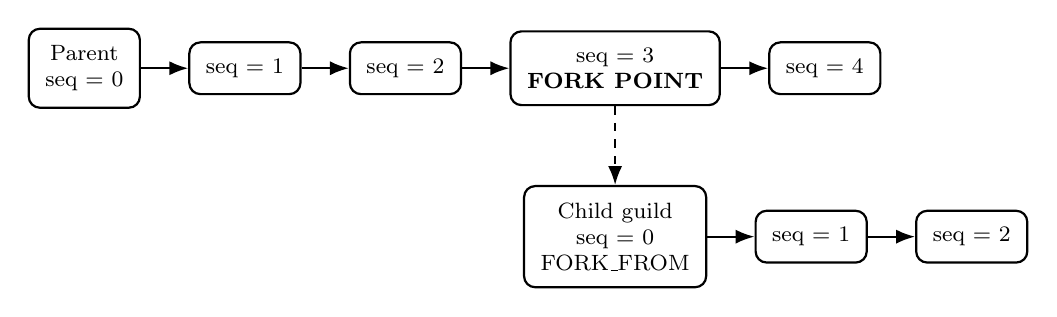
\begin{tikzpicture}[node distance=6mm]
\node[box] (p0) {Parent\\seq = 0};
\node[box, right=6mm of p0] (p1) {seq = 1};
\node[box, right=6mm of p1] (p2) {seq = 2};
\node[box, right=6mm of p2] (pf) {seq = 3\\\textbf{FORK POINT}};
\node[box, right=6mm of pf] (p4) {seq = 4};

\node[box, below=10mm of pf] (c0) {Child guild\\seq = 0\\FORK\_FROM};
\node[box, right=6mm of c0] (c1) {seq = 1};
\node[box, right=6mm of c1] (c2) {seq = 2};

\draw[arr] (p0) -- (p1);
\draw[arr] (p1) -- (p2);
\draw[arr] (p2) -- (pf);
\draw[darr] (pf) -- (c0);
\draw[arr] (pf) -- (p4);
\draw[arr] (c0) -- (c1);
\draw[arr] (c1) -- (c2);
\end{tikzpicture}%
}
\caption{Forking: a new guild log can branch from a parent at a verifiable checkpoint. Clients can present forks as alternative histories with shared provenance rather than hidden conflicts.}
\label{fig:fork}
\end{figure}

\newpage
\textbf{Explicit exit via forks.} While forks exist socially in many ecosystems, \cgp makes forking a first-class governance action encoded in the log. This makes community splits legible to clients, rather than being hidden in out-of-band coordination (Figure \ref{fig:fork}).

\medskip
\noindent\textit{B. Relation to neighboring designs.}

\textbf{Relation to Git-style DVCS and hosting.}
A \cgp guild log resembles a Git repository: both are append-only histories with signed updates and explicit forks, and both can be hosted by third parties.
Git hosting platforms (e.g., GitHub) bundle naming, hosting, and access control into a single service.
\cgp instead splits these concerns across relay roles: directory operators implement a transparent naming and discovery role, guild relays sequence chat events, and optional media or policy relays.
This unbundling lets communities move or replicate each role independently while keeping chat and governance semantics tailored to guilds rather than code.

\textbf{Relation to Nostr and NIPs.}
Nostr standardizes a generic event + relay model and leaves richer semantics to optional Nostr Improvement Protocols (NIPs) \cite{nostrNIP01}.
\cgp, by contrast, depends on per-guild, hash-linked logs, CT-style directory transparency, and explicit relay roles.
While these could be approximated as a Nostr profile, they require CGP-specific relay behavior and rules that go beyond Nostr's ``dumb relay'' philosophy, so we specify \cgp as a separate guild-centric protocol rather than as a NIP.


\section{Massive Data and Rich Media (MP4, Attachments, Archives)}
Large binaries stress any messaging system. Centralized platforms typically enforce upload caps and rely on HTTP caching / edge delivery infrastructure for attachments \cite{rfc7234}. Matrix places storage and serving responsibilities on homeserver operators as part of its federated design \cite{jacob2020matrixdecomposition}. The \atproto separates signed records from content-addressed blobs, keeping large media out of the repository history \cite{kleppmann2024atproto}.  In \cgp, we follow this separation-of-concerns approach explicitly, treating rich media as a distinct plane that can scale and evolve independently of the guild log.

\subsection{CGP approach: keep the log small and media pluggable}
We recommend treating media as separate \emph{blob objects} referenced from log events by content hash plus metadata (MIME type, size, and optional thumbnails). This aligns with content-addressed storage and deduplication principles used in systems such as IPFS \cite{ipfs} and \atproto \cite{atprotoBlobSpec}. We couple this system with optional relay plugins and show the pipeline in Figure \ref{fig:media}.

\subsection{Scaling considerations}
\textbf{Streaming video.} For MP4 and long-form video, \cgp clients can prefer manifests (HLS/DASH) represented as blob sets, with the log referencing the manifest root hash and track hashes. This prevents ``messages as megabytes'' attacks while enabling partial retrieval.

\textbf{Retention and cost.} Centralized platforms often monetize higher resource limits via subscription tiers (e.g., Discord’s Nitro/boost model) \cite{robinson2022yeet}. \cgp can support similar cost controls \emph{without} central ownership by letting relays declare and enforce policies: (1) maximum blob size per guild; (2) time-to-live (TTL) for unpinned blobs; and (3) optional pay-by-resource plugins, while keeping the base standard tokenless.

\textbf{Archival exports.} Logs can be exported as compact, verified sequences. Blobs can be exported as CAR-like bundles (as in \atproto repositories \cite{atprotoRepoSpec}) or as content-addressed directories (IPFS-style) \cite{ipfs}.

\section{Security and Trust Model}
\subsection{Tamper evidence and equivocation}
Hash-linked logs make rewrites detectable once a client has seen any checkpoint. However, a malicious relay could \emph{equivocate} by serving different log heads to different clients. \cgp mitigates this with: (i) client cross-checking across relays (multiple relays per guild), (ii) explicit checkpoints that are signed and optionally anchored, and (iii) directory transparency that can reveal inconsistent claims using consistency proofs \cite{rfc6962}.

\subsection{Optional anchoring: checkpoints on-chain}
\cgp does not require a blockchain but can harden history by anchoring (a) directory Merkle roots and/or (b) guild log root hashes. A practical method is to commit small hashes into Bitcoin transactions using null-data outputs (OP\_RETURN) \cite{nakamoto2008bitcoin}. Anchoring can be implemented by periodically publishing a checkpoint commitment into a public blockchain transaction, using Merkle batching to amortize cost across many checkpoints \cite{haber1991timestamping,merkle1987,nakamoto2008bitcoin}.

\subsection{Spam, Sybils, and abuse}
Rather than mandating a universal mechanism, \cgp treats anti-abuse as a \emph{relay policy plugin surface}. Options include: proof-of-work gating (e.g., Hashcash-style puzzles) \cite{hashcash2}; rate limits (e.g., HTTP 429 ``Too Many Requests'') \cite{rfc6585}; membership proofs (invite codes, WebAuthn, or reputation signals); and bandwidth or compression budgets, as discussed below.

\begin{figure}[t]
\centering
\resizebox{\columnwidth}{!}{%
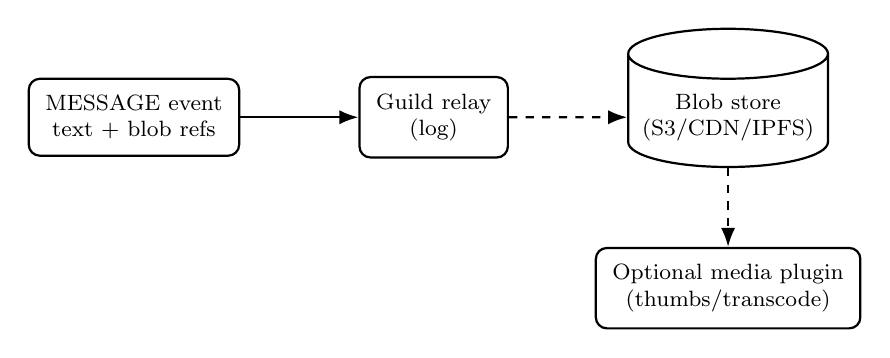
\begin{tikzpicture}[node distance=10mm]

\node[box] (msg) {MESSAGE event\\text + blob refs};
\node[box, right=15mm of msg] (relay) {Guild relay\\(log)};
\node[db,  right=15mm of relay] (blob) {Blob store\\(S3/CDN/IPFS)};
\node[box, below=10mm of blob] (transcode) {Optional media plugin\\(thumbs/transcode)};

% simple arrows, no labels
\draw[arr]  (msg)   -- (relay);
\draw[darr] (relay) -- (blob);
\draw[darr] (blob)  -- (transcode);

\end{tikzpicture}%
}
\caption{Recommended media plane. Logs remain compact; events reference blobs by hash or CID; optional plugins add thumbnails, transcoding, or pinning policies.}
\label{fig:media}
\end{figure}

\section{Future Work}
\subsection{Proof-of-work (optional, per relay)}
Proof-of-work (PoW) can deter spam in open relays without requiring tokens. A relay could require a lightweight Hashcash token for \texttt{PUBLISH} requests in high-risk channels \cite{hashcash2}. Importantly, this remains configurable: small private guilds can disable PoW entirely, and public megaguilds can enable it only for new accounts or suspicious bursts.

\subsection{Proof-of-compression and ``bandwidth fairness''}
A distinctive extension is \emph{proof-of-compression}: rather than charging money, a relay can require that large payloads (e.g., pasted logs, images, short clips) be accompanied by: (1) deterministic compression parameters (codec and level); (2) a commitment to the compressed bytes (hash or CID); and (3) a verifier rule that checks the compressed artifact meets target size bounds. This creates a ``cost'' denominated in user time and compute rather than currency. For more cryptographic rigor, one can explore succinct proofs and commitment schemes, but a practical first step is deterministic compression plus hash commitments and sampling audits.

\subsection{Proof-of-retention for relays (auditable storage)}
Large guilds will want assurances about what relays actually retain. Proofs of Retrievability (PoR) and Provable Data Possession (PDP) provide foundations for verifying that an untrusted storage provider still holds content \cite{juels2007por,ateniese2007pdp}. A \cgp ``retention plugin'' could challenge relays to produce probabilistic proofs for log ranges and pinned blobs, creating a verifiable service-level agreement (SLA) without requiring a blockchain.

\subsection{Checkpointing conversation histories on-chain}
We envision two complementary checkpointing strategies: (i) directory-root anchoring for handle integrity via periodic Merkle roots \cite{rfc6962}; and (ii) guild-root anchoring for chat history via periodic log-head hashes. Anchoring can be done directly via Bitcoin null-data outputs \cite{bitcoinDevTx} or via timestamping systems (e.g., OpenTimestamps batching) \cite{opentimestamps,opentimestampsTodd}. Clients can then show ``verified as of block height $X$'' for sensitive governance events (bans, elections, forks).

\subsection{Media sharding and interoperability with CDNs}
Commercial chat systems typically centralize attachment hosting and enforce plan- or policy-based limits. \cgp can replicate similar UX while remaining protocol-neutral by standardizing: (1) a blob-reference schema (hash plus metadata); (2) an optional ``media relay'' role; and (3) transform attestations (thumbnail/transcode hashes). This mirrors \atproto's explicit separation of records from blobs \cite{atprotoBlobSpec,atprotoRepoSpec} while allowing alternate backends such as S3-compatible stores, IPFS pinsets \cite{ipfs}, or community-operated CDNs.

\section{Conclusion}
\cgp targets a pragmatic point in the design space: guild-style group chat with verifiable history and forkable governance, without imposing tokens, mining, or mandatory global consensus. By combining append-only signed logs with transparency-based discovery and a role-based relay architecture, \cgp provides a foundation for interoperable UX while keeping policy extensible through optional relay roles and plugins. Future work can add selective proofs (PoW, compression, retention), scalable media planes, and optional on-chain checkpointing for high-integrity communities.

\balance
\bibliographystyle{IEEEtran}
\bibliography{references}

\end{document}
